%% fig_closure.tex   (generated by make_closure.py; do not edit by hand)
%% The route of this paper through the rule set of the closure theorem, as a stack of plates, one per level of the derivation.
\documentclass[tikz,border=8pt]{standalone}
\usepackage{amsmath,amssymb}
\usetikzlibrary{arrows.meta,calc,decorations.pathreplacing}
%% palette.tex -- shared colour definitions for the figures
\definecolor{PInk}{RGB}{26,32,44}
\definecolor{PBlue}{RGB}{37,82,139}
\definecolor{PTeal}{RGB}{23,127,125}
\definecolor{POchre}{RGB}{193,138,44}
\definecolor{PClay}{RGB}{178,74,58}
\definecolor{PSlate}{RGB}{108,122,137}
\definecolor{PViolet}{RGB}{110,86,150}
\definecolor{WBlue}{RGB}{223,234,246}
\definecolor{WTeal}{RGB}{220,238,236}
\definecolor{WOchre}{RGB}{250,240,218}
\definecolor{WClay}{RGB}{247,229,224}
\definecolor{WSlate}{RGB}{238,241,244}
\definecolor{PMag}{RGB}{158,58,110}
\definecolor{PGrass}{RGB}{62,124,66}
\definecolor{PAmber}{RGB}{214,112,38}
\definecolor{PIndigo}{RGB}{58,64,140}
\definecolor{PRule}{RGB}{176,186,197}

%% shared macros so the standalone figures match the paper
\providecommand{\QQ}{\mathbb{Q}}
\providecommand{\ZZ}{\mathbb{Z}}
\providecommand{\RR}{\mathbb{R}}
\providecommand{\CC}{\mathbb{C}}
\providecommand{\PP}{\mathbb{P}}
\providecommand{\Kx}{K^{\times}}
\providecommand{\HW}{W}
\providecommand{\Nm}{\mathrm{N}}
\providecommand{\Hdg}{\mathrm{Hdg}}
\providecommand{\NS}{\mathrm{NS}}
\providecommand{\cA}{\mathcal{A}}
\providecommand{\cD}{\mathcal{D}}
\providecommand{\cF}{\mathcal{F}}
\providecommand{\cP}{\mathcal{P}}
\providecommand{\cO}{\mathcal{O}}
\providecommand{\cQ}{\mathcal{Q}}
\providecommand{\bbar}[1]{\overline{#1}}
\providecommand{\ch}{\operatorname{ch}}
\providecommand{\End}{\mathrm{End}}
\providecommand{\Ext}{\operatorname{Ext}}
\providecommand{\Supp}{\operatorname{Supp}}

\begin{document}
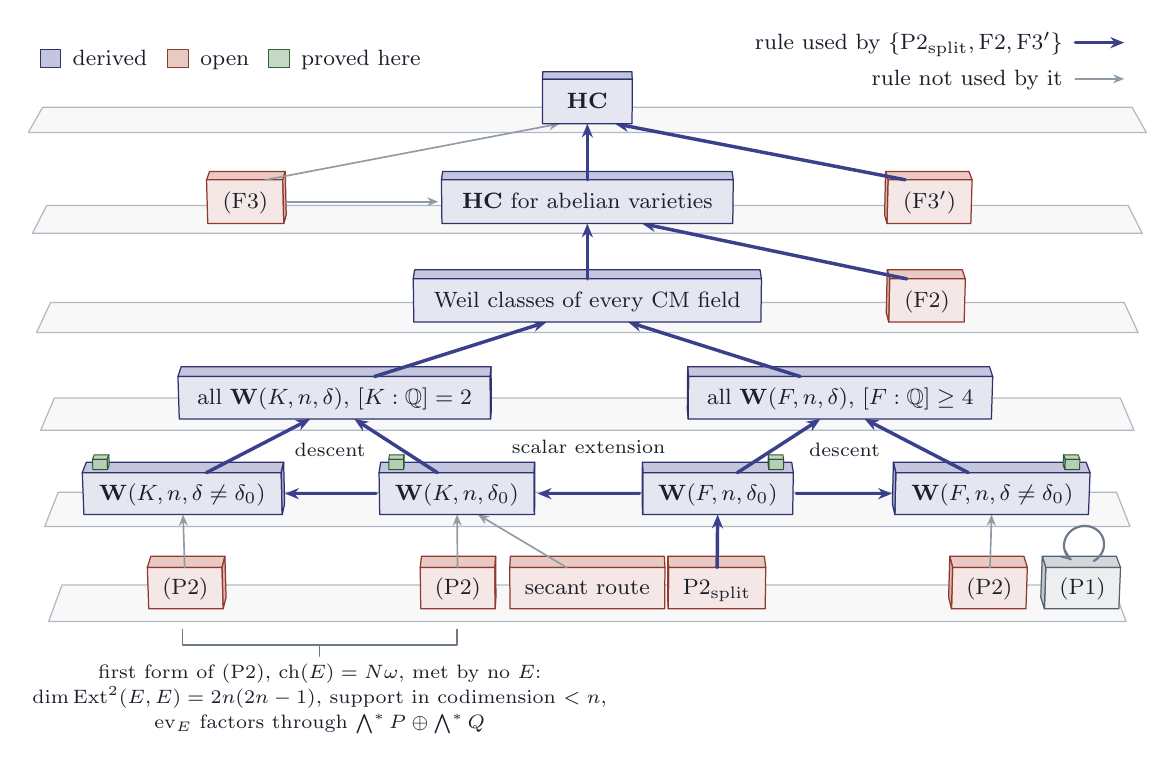
\begin{tikzpicture}[x=1cm,y=1cm,line join=round,line cap=round,
  font=\small,text=PInk,lbl/.style={inner sep=1pt}]
  \colorlet{FFd}{PIndigo!13!white}
  \colorlet{FFo}{PClay!13!white}
  \colorlet{FFp}{PGrass!13!white}
  \colorlet{FFs}{PSlate!13!white}
  \path[fill=PSlate!5,draw=PRule,line width=0.45pt] (-6.8417,-3.0638) -- (6.8417,-3.0638) -- (6.6723,-2.6002) -- (-6.6723,-2.6002) -- cycle;
  \path[fill=PSlate!30!white,draw=PSlate!80!black,line width=0.45pt] (5.8225,-2.3775) -- (6.7714,-2.3775) -- (6.7184,-2.2363) -- (5.7769,-2.2363) -- cycle;
  \path[fill=FFs,draw=PSlate!80!black,line width=0.45pt] (5.8040,-2.9018) -- (6.7499,-2.9018) -- (6.7714,-2.3775) -- (5.8225,-2.3775) -- cycle;
  \path[fill=PSlate!42!white,draw=PSlate!80!black,line width=0.45pt] (5.8040,-2.9018) -- (5.7587,-2.7569) -- (5.7769,-2.2363) -- (5.8225,-2.3775) -- cycle;
  \path[fill=PClay!30!white,draw=PClay!80!black,line width=0.45pt] (-5.5881,-2.3775) -- (-4.6392,-2.3775) -- (-4.6028,-2.2363) -- (-5.5443,-2.2363) -- cycle;
  \path[fill=FFo,draw=PClay!80!black,line width=0.45pt] (-5.5703,-2.9018) -- (-4.6244,-2.9018) -- (-4.6392,-2.3775) -- (-5.5881,-2.3775) -- cycle;
  \path[fill=PClay!42!white,draw=PClay!80!black,line width=0.45pt] (-4.6244,-2.9018) -- (-4.5883,-2.7569) -- (-4.6028,-2.2363) -- (-4.6392,-2.3775) -- cycle;
  \path[fill=PClay!30!white,draw=PClay!80!black,line width=0.45pt] (4.6392,-2.3775) -- (5.5881,-2.3775) -- (5.5443,-2.2363) -- (4.6028,-2.2363) -- cycle;
  \path[fill=FFo,draw=PClay!80!black,line width=0.45pt] (4.6244,-2.9018) -- (5.5703,-2.9018) -- (5.5881,-2.3775) -- (4.6392,-2.3775) -- cycle;
  \path[fill=PClay!42!white,draw=PClay!80!black,line width=0.45pt] (4.6244,-2.9018) -- (4.5883,-2.7569) -- (4.6028,-2.2363) -- (4.6392,-2.3775) -- cycle;
  \path[fill=PClay!30!white,draw=PClay!80!black,line width=0.45pt] (-2.1226,-2.3775) -- (-1.1737,-2.3775) -- (-1.1645,-2.2363) -- (-2.1060,-2.2363) -- cycle;
  \path[fill=FFo,draw=PClay!80!black,line width=0.45pt] (-2.1159,-2.9018) -- (-1.1700,-2.9018) -- (-1.1737,-2.3775) -- (-2.1226,-2.3775) -- cycle;
  \path[fill=PClay!42!white,draw=PClay!80!black,line width=0.45pt] (-1.1700,-2.9018) -- (-1.1609,-2.7569) -- (-1.1645,-2.2363) -- (-1.1737,-2.3775) -- cycle;
  \path[fill=PClay!30!white,draw=PClay!80!black,line width=0.45pt] (1.0307,-2.3775) -- (2.2657,-2.3775) -- (2.2480,-2.2363) -- (1.0226,-2.2363) -- cycle;
  \path[fill=FFo,draw=PClay!80!black,line width=0.45pt] (1.0274,-2.9018) -- (2.2585,-2.9018) -- (2.2657,-2.3775) -- (1.0307,-2.3775) -- cycle;
  \path[fill=PClay!42!white,draw=PClay!80!black,line width=0.45pt] (1.0274,-2.9018) -- (1.0194,-2.7569) -- (1.0226,-2.2363) -- (1.0307,-2.3775) -- cycle;
  \path[fill=PClay!30!white,draw=PClay!80!black,line width=0.45pt] (-0.9854,-2.3775) -- (0.9854,-2.3775) -- (0.9777,-2.2363) -- (-0.9777,-2.2363) -- cycle;
  \path[fill=FFo,draw=PClay!80!black,line width=0.45pt] (-0.9823,-2.9018) -- (0.9823,-2.9018) -- (0.9854,-2.3775) -- (-0.9854,-2.3775) -- cycle;
  \path[fill=PSlate!5,draw=PRule,line width=0.45pt] (-6.8918,-1.8581) -- (6.8918,-1.8581) -- (6.7200,-1.4213) -- (-6.7200,-1.4213) -- cycle;
  \draw[PSlate!75,line width=0.6pt,-{Stealth[length=4pt,width=3.2pt]}] (-5.1136,-2.3775) -- (-5.1344,-1.7055);
  \draw[PSlate!75,line width=0.6pt,-{Stealth[length=4pt,width=3.2pt]}] (-1.6482,-2.3775) -- (-1.6549,-1.7055);
  \draw[PIndigo,line width=1.25pt,-{Stealth[length=5pt,width=4pt]}] (1.6482,-2.3775) -- (1.6549,-1.7055);
  \draw[PSlate!75,line width=0.6pt,-{Stealth[length=4pt,width=3.2pt]}] (5.1136,-2.3775) -- (5.1344,-1.7055);
  \draw[PSlate!75,line width=0.6pt,-{Stealth[length=4pt,width=3.2pt]}] (-0.2637,-2.3775) -- (-1.3901,-1.7055);
  \path[fill=PIndigo!30!white,draw=PIndigo!80!black,line width=0.45pt] (-6.4141,-1.1736) -- (-3.8877,-1.1736) -- (-3.8570,-1.0409) -- (-6.3635,-1.0409) -- cycle;
  \path[fill=FFd,draw=PIndigo!80!black,line width=0.45pt] (-6.3936,-1.7055) -- (-3.8752,-1.7055) -- (-3.8877,-1.1736) -- (-6.4141,-1.1736) -- cycle;
  \path[fill=PIndigo!42!white,draw=PIndigo!80!black,line width=0.45pt] (-3.8752,-1.7055) -- (-3.8448,-1.5690) -- (-3.8570,-1.0409) -- (-3.8877,-1.1736) -- cycle;
  \path[fill=PGrass!33!white,draw=PGrass!70!black,line width=0.35pt] (-6.2848,-1.0044) -- (-6.0978,-1.0044) -- (-6.0766,-0.9464) -- (-6.2630,-0.9464) -- cycle;
  \path[fill=PGrass!38!white,draw=PGrass!70!black,line width=0.35pt] (-6.2799,-1.1336) -- (-6.0931,-1.1336) -- (-6.0978,-1.0044) -- (-6.2848,-1.0044) -- cycle;
  \path[fill=PGrass!46!white,draw=PGrass!70!black,line width=0.35pt] (-6.0931,-1.1336) -- (-6.0719,-1.0752) -- (-6.0766,-0.9464) -- (-6.0978,-1.0044) -- cycle;
  \path[fill=PIndigo!30!white,draw=PIndigo!80!black,line width=0.45pt] (3.9174,-1.1736) -- (6.3844,-1.1736) -- (6.3341,-1.0409) -- (3.8865,-1.0409) -- cycle;
  \path[fill=FFd,draw=PIndigo!80!black,line width=0.45pt] (3.9049,-1.7055) -- (6.3640,-1.7055) -- (6.3844,-1.1736) -- (3.9174,-1.1736) -- cycle;
  \path[fill=PIndigo!42!white,draw=PIndigo!80!black,line width=0.45pt] (3.9049,-1.7055) -- (3.8742,-1.5690) -- (3.8865,-1.0409) -- (3.9174,-1.1736) -- cycle;
  \path[fill=PGrass!33!white,draw=PGrass!70!black,line width=0.35pt] (6.0682,-1.0044) -- (6.2552,-1.0044) -- (6.2334,-0.9464) -- (6.0470,-0.9464) -- cycle;
  \path[fill=PGrass!38!white,draw=PGrass!70!black,line width=0.35pt] (6.0634,-1.1336) -- (6.2503,-1.1336) -- (6.2552,-1.0044) -- (6.0682,-1.0044) -- cycle;
  \path[fill=PGrass!61!white,draw=PGrass!70!black,line width=0.35pt] (6.0634,-1.1336) -- (6.0424,-1.0752) -- (6.0470,-0.9464) -- (6.0682,-1.0044) -- cycle;
  \path[fill=PIndigo!30!white,draw=PIndigo!80!black,line width=0.45pt] (-2.6455,-1.1736) -- (-0.6749,-1.1736) -- (-0.6696,-1.0409) -- (-2.6247,-1.0409) -- cycle;
  \path[fill=FFd,draw=PIndigo!80!black,line width=0.45pt] (-2.6371,-1.7055) -- (-0.6727,-1.7055) -- (-0.6749,-1.1736) -- (-2.6455,-1.1736) -- cycle;
  \path[fill=PIndigo!42!white,draw=PIndigo!80!black,line width=0.45pt] (-0.6727,-1.7055) -- (-0.6674,-1.5690) -- (-0.6696,-1.0409) -- (-0.6749,-1.1736) -- cycle;
  \path[fill=PGrass!33!white,draw=PGrass!70!black,line width=0.35pt] (-2.5223,-1.0044) -- (-2.3353,-1.0044) -- (-2.3271,-0.9464) -- (-2.5135,-0.9464) -- cycle;
  \path[fill=PGrass!38!white,draw=PGrass!70!black,line width=0.35pt] (-2.5203,-1.1336) -- (-2.3335,-1.1336) -- (-2.3353,-1.0044) -- (-2.5223,-1.0044) -- cycle;
  \path[fill=PGrass!46!white,draw=PGrass!70!black,line width=0.35pt] (-2.3335,-1.1336) -- (-2.3253,-1.0752) -- (-2.3271,-0.9464) -- (-2.3353,-1.0044) -- cycle;
  \path[fill=PIndigo!30!white,draw=PIndigo!80!black,line width=0.45pt] (0.7046,-1.1736) -- (2.6158,-1.1736) -- (2.5952,-1.0409) -- (0.6990,-1.0409) -- cycle;
  \path[fill=FFd,draw=PIndigo!80!black,line width=0.45pt] (0.7023,-1.7055) -- (2.6074,-1.7055) -- (2.6158,-1.1736) -- (0.7046,-1.1736) -- cycle;
  \path[fill=PIndigo!42!white,draw=PIndigo!80!black,line width=0.45pt] (0.7023,-1.7055) -- (0.6968,-1.5690) -- (0.6990,-1.0409) -- (0.7046,-1.1736) -- cycle;
  \path[fill=PGrass!33!white,draw=PGrass!70!black,line width=0.35pt] (2.3056,-1.0044) -- (2.4926,-1.0044) -- (2.4839,-0.9464) -- (2.2976,-0.9464) -- cycle;
  \path[fill=PGrass!38!white,draw=PGrass!70!black,line width=0.35pt] (2.3038,-1.1336) -- (2.4907,-1.1336) -- (2.4926,-1.0044) -- (2.3056,-1.0044) -- cycle;
  \path[fill=PGrass!61!white,draw=PGrass!70!black,line width=0.35pt] (2.3038,-1.1336) -- (2.2958,-1.0752) -- (2.2976,-0.9464) -- (2.3056,-1.0044) -- cycle;
  \draw[PIndigo,line width=1.25pt,-{Stealth[length=5pt,width=4pt]}] (-2.6838,-1.4400) -- (-3.8389,-1.4400);
  \draw[PIndigo,line width=1.25pt,-{Stealth[length=5pt,width=4pt]}] (2.6541,-1.4400) -- (3.8686,-1.4400);
  \draw[PIndigo,line width=1.25pt,-{Stealth[length=5pt,width=4pt]}] (0.6610,-1.4400) -- (-0.6313,-1.4400);
  \path[fill=PSlate!5,draw=PRule,line width=0.45pt] (-6.9427,-0.6347) -- (6.9427,-0.6347) -- (6.7683,-0.2255) -- (-6.7683,-0.2255) -- cycle;
  \draw[PIndigo,line width=1.25pt,-{Stealth[length=5pt,width=4pt]}] (-4.8376,-1.1736) -- (-3.5204,-0.4917);
  \draw[PIndigo,line width=1.25pt,-{Stealth[length=5pt,width=4pt]}] (-1.9054,-1.1736) -- (-2.9596,-0.4917);
  \draw[PIndigo,line width=1.25pt,-{Stealth[length=5pt,width=4pt]}] (1.9054,-1.1736) -- (2.9596,-0.4917);
  \draw[PIndigo,line width=1.25pt,-{Stealth[length=5pt,width=4pt]}] (4.8376,-1.1736) -- (3.5204,-0.4917);
  \path[fill=PIndigo!30!white,draw=PIndigo!80!black,line width=0.45pt] (-5.1994,0.0480) -- (-1.2329,0.0480) -- (-1.2231,0.1720) -- (-5.1581,0.1720) -- cycle;
  \path[fill=FFd,draw=PIndigo!80!black,line width=0.45pt] (-5.1826,-0.4917) -- (-1.2290,-0.4917) -- (-1.2329,0.0480) -- (-5.1994,0.0480) -- cycle;
  \path[fill=PIndigo!42!white,draw=PIndigo!80!black,line width=0.45pt] (-1.2290,-0.4917) -- (-1.2192,-0.3638) -- (-1.2231,0.1720) -- (-1.2329,0.0480) -- cycle;
  \path[fill=PIndigo!30!white,draw=PIndigo!80!black,line width=0.45pt] (1.2842,0.0480) -- (5.1481,0.0480) -- (5.1072,0.1720) -- (1.2740,0.1720) -- cycle;
  \path[fill=FFd,draw=PIndigo!80!black,line width=0.45pt] (1.2801,-0.4917) -- (5.1315,-0.4917) -- (5.1481,0.0480) -- (1.2842,0.0480) -- cycle;
  \path[fill=PIndigo!42!white,draw=PIndigo!80!black,line width=0.45pt] (1.2801,-0.4917) -- (1.2699,-0.3638) -- (1.2740,0.1720) -- (1.2842,0.0480) -- cycle;
  \path[fill=PSlate!5,draw=PRule,line width=0.45pt] (-6.9944,0.6069) -- (6.9944,0.6069) -- (6.8174,0.9877) -- (-6.8174,0.9877) -- cycle;
  \draw[PIndigo,line width=1.25pt,-{Stealth[length=5pt,width=4pt]}] (-2.7016,0.0480) -- (-0.5167,0.7400);
  \draw[PIndigo,line width=1.25pt,-{Stealth[length=5pt,width=4pt]}] (2.7016,0.0480) -- (0.5167,0.7400);
  \path[fill=PClay!30!white,draw=PClay!80!black,line width=0.45pt] (3.8393,1.2877) -- (4.8006,1.2877) -- (4.7622,1.4027) -- (3.8085,1.4027) -- cycle;
  \path[fill=FFo,draw=PClay!80!black,line width=0.45pt] (3.8268,0.7400) -- (4.7850,0.7400) -- (4.8006,1.2877) -- (3.8393,1.2877) -- cycle;
  \path[fill=PClay!42!white,draw=PClay!80!black,line width=0.45pt] (3.8268,0.7400) -- (3.7963,0.8590) -- (3.8085,1.4027) -- (3.8393,1.2877) -- cycle;
  \path[fill=PIndigo!30!white,draw=PIndigo!80!black,line width=0.45pt] (-2.2112,1.2877) -- (2.2112,1.2877) -- (2.1935,1.4027) -- (-2.1935,1.4027) -- cycle;
  \path[fill=FFd,draw=PIndigo!80!black,line width=0.45pt] (-2.2040,0.7400) -- (2.2040,0.7400) -- (2.2112,1.2877) -- (-2.2112,1.2877) -- cycle;
  \path[fill=PSlate!5,draw=PRule,line width=0.45pt] (-7.0468,1.8671) -- (7.0468,1.8671) -- (6.8672,2.2186) -- (-6.8672,2.2186) -- cycle;
  \draw[PIndigo,line width=1.25pt,-{Stealth[length=5pt,width=4pt]}] (0.0000,1.2877) -- (0.0000,1.9900);
  \draw[PIndigo,line width=1.25pt,-{Stealth[length=5pt,width=4pt]}] (4.0553,1.2877) -- (0.6941,1.9900);
  \path[fill=PClay!30!white,draw=PClay!80!black,line width=0.45pt] (-4.8364,2.5459) -- (-3.8679,2.5459) -- (-3.8367,2.6516) -- (-4.7974,2.6516) -- cycle;
  \path[fill=FFo,draw=PClay!80!black,line width=0.45pt] (-4.8206,1.9900) -- (-3.8552,1.9900) -- (-3.8679,2.5459) -- (-4.8364,2.5459) -- cycle;
  \path[fill=PClay!42!white,draw=PClay!80!black,line width=0.45pt] (-3.8552,1.9900) -- (-3.8243,2.0998) -- (-3.8367,2.6516) -- (-3.8679,2.5459) -- cycle;
  \path[fill=PClay!30!white,draw=PClay!80!black,line width=0.45pt] (3.8181,2.5459) -- (4.8861,2.5459) -- (4.8467,2.6516) -- (3.7874,2.6516) -- cycle;
  \path[fill=FFo,draw=PClay!80!black,line width=0.45pt] (3.8057,1.9900) -- (4.8701,1.9900) -- (4.8861,2.5459) -- (3.8181,2.5459) -- cycle;
  \path[fill=PClay!42!white,draw=PClay!80!black,line width=0.45pt] (3.8057,1.9900) -- (3.7751,2.0998) -- (3.7874,2.6516) -- (3.8181,2.5459) -- cycle;
  \path[fill=PIndigo!30!white,draw=PIndigo!80!black,line width=0.45pt] (-1.8530,2.5459) -- (1.8530,2.5459) -- (1.8381,2.6516) -- (-1.8381,2.6516) -- cycle;
  \path[fill=FFd,draw=PIndigo!80!black,line width=0.45pt] (-1.8469,1.9900) -- (1.8469,1.9900) -- (1.8530,2.5459) -- (-1.8530,2.5459) -- cycle;
  \draw[PSlate!75,line width=0.6pt,-{Stealth[length=4pt,width=3.2pt]}] (-3.8181,2.2675) -- (-1.8934,2.2675);
  \path[fill=PSlate!5,draw=PRule,line width=0.45pt] (-7.1000,3.1464) -- (7.1000,3.1464) -- (6.9177,3.4676) -- (-6.9177,3.4676) -- cycle;
  \draw[PIndigo,line width=1.25pt,-{Stealth[length=5pt,width=4pt]}] (0.0000,2.5459) -- (0.0000,3.2587);
  \draw[PIndigo,line width=1.25pt,-{Stealth[length=5pt,width=4pt]}] (4.0357,2.5459) -- (0.3496,3.2587);
  \draw[PSlate!75,line width=0.6pt,-{Stealth[length=4pt,width=3.2pt]}] (-4.0855,2.5459) -- (-0.3496,3.2587);
  \path[fill=PIndigo!30!white,draw=PIndigo!80!black,line width=0.45pt] (-0.5700,3.8230) -- (0.5700,3.8230) -- (0.5654,3.9191) -- (-0.5654,3.9191) -- cycle;
  \path[fill=FFd,draw=PIndigo!80!black,line width=0.45pt] (-0.5681,3.2587) -- (0.5681,3.2587) -- (0.5700,3.8230) -- (-0.5700,3.8230) -- cycle;
  \draw[PSlate,line width=0.8pt,-{Stealth[length=4pt,width=3.2pt]}] (6.4327,-2.2944) -- (6.4551,-2.2802) -- (6.4760,-2.2640) -- (6.4950,-2.2458) -- (6.5119,-2.2259) -- (6.5266,-2.2045) -- (6.5390,-2.1819) -- (6.5488,-2.1582) -- (6.5559,-2.1338) -- (6.5604,-2.1090) -- (6.5621,-2.0839) -- (6.5610,-2.0588) -- (6.5571,-2.0341) -- (6.5505,-2.0100) -- (6.5412,-1.9868) -- (6.5294,-1.9647) -- (6.5151,-1.9440) -- (6.4986,-1.9249) -- (6.4800,-1.9075) -- (6.4594,-1.8922) -- (6.4372,-1.8791) -- (6.4136,-1.8682) -- (6.3889,-1.8598) -- (6.3632,-1.8540) -- (6.3369,-1.8507) -- (6.3103,-1.8500) -- (6.2837,-1.8520) -- (6.2574,-1.8566) -- (6.2316,-1.8638) -- (6.2066,-1.8734) -- (6.1828,-1.8854) -- (6.1603,-1.8997) -- (6.1395,-1.9160) -- (6.1205,-1.9343) -- (6.1035,-1.9542) -- (6.0888,-1.9757) -- (6.0766,-1.9984) -- (6.0668,-2.0221) -- (6.0597,-2.0465) -- (6.0553,-2.0714) -- (6.0537,-2.0965) -- (6.0549,-2.1215) -- (6.0589,-2.1462) -- (6.0655,-2.1703) -- (6.0749,-2.1934) -- (6.0867,-2.2155) -- (6.1010,-2.2361) -- (6.1176,-2.2552) -- (6.1362,-2.2724) -- (6.1567,-2.2877);
  \draw[PSlate,line width=0.5pt] (-5.1419,-3.1638) -- (-5.1419,-3.3638) -- (-1.6573,-3.3638) -- (-1.6573,-3.1638);
  \draw[PSlate,line width=0.5pt] (-3.3996,-3.3638) -- (-3.3996,-3.5038);
  \path[fill=PIndigo!30!white,draw=PIndigo!80!black,line width=0.4pt] (-6.9477,3.9776) rectangle (-6.6877,4.1976);
  \path[fill=PClay!30!white,draw=PClay!80!black,line width=0.4pt] (-5.3277,3.9776) rectangle (-5.0677,4.1976);
  \path[fill=PGrass!30!white,draw=PGrass!80!black,line width=0.4pt] (-4.0477,3.9776) rectangle (-3.7877,4.1976);
  \draw[PIndigo,line width=1.25pt,-{Stealth[length=5pt,width=4pt]}] (6.1977,4.2876) -- (6.8177,4.2876);
  \draw[PSlate!75,line width=0.6pt,-{Stealth[length=4pt,width=3.2pt]}] (6.1977,3.8276) -- (6.8177,3.8276);
  \node[lbl,text=PInk,font=\footnotesize,text height=1.6ex,text depth=0.45ex] at (0.0000,3.5404) {$\mathbf{HC}$};
  \node[lbl,text=PInk,font=\footnotesize,text height=1.6ex,text depth=0.45ex] at (0.0000,2.2675) {$\mathbf{HC}$ for abelian varieties};
  \node[lbl,text=PInk,font=\footnotesize,text height=1.6ex,text depth=0.45ex] at (-4.3450,2.2675) {(F3)};
  \node[lbl,text=PInk,font=\footnotesize,text height=1.6ex,text depth=0.45ex] at (4.3450,2.2675) {(F3$'$)};
  \node[lbl,text=PInk,font=\footnotesize,text height=1.6ex,text depth=0.45ex] at (0.0000,1.0134) {Weil classes of every CM field};
  \node[lbl,text=PInk,font=\footnotesize,text height=1.6ex,text depth=0.45ex] at (4.3129,1.0134) {(F2)};
  \node[lbl,text=PInk,font=\footnotesize,text height=1.6ex,text depth=0.45ex] at (-3.2110,-0.2223) {all $\mathbf{W}(K,n,\delta)$, $[K:\mathbb{Q}]=2$};
  \node[lbl,text=PInk,font=\footnotesize,text height=1.6ex,text depth=0.45ex] at (3.2110,-0.2223) {all $\mathbf{W}(F,n,\delta)$, $[F:\mathbb{Q}]\ge4$};
  \node[lbl,text=PInk,font=\footnotesize,text height=1.6ex,text depth=0.45ex] at (-5.1426,-1.4400) {$\mathbf{W}(K,n,\delta\neq\delta_{0})$};
  \node[lbl,text=PInk,font=\footnotesize,text height=1.6ex,text depth=0.45ex] at (-1.6575,-1.4400) {$\mathbf{W}(K,n,\delta_{0})$};
  \node[lbl,text=PInk,font=\footnotesize,text height=1.6ex,text depth=0.45ex] at (1.6575,-1.4400) {$\mathbf{W}(F,n,\delta_{0})$};
  \node[lbl,text=PInk,font=\footnotesize,text height=1.6ex,text depth=0.45ex] at (5.1426,-1.4400) {$\mathbf{W}(F,n,\delta\neq\delta_{0})$};
  \node[lbl,text=PInk,font=\footnotesize,text height=1.6ex,text depth=0.45ex] at (-5.1055,-2.6401) {(P2)};
  \node[lbl,text=PInk,font=\footnotesize,text height=1.6ex,text depth=0.45ex] at (-1.6456,-2.6401) {(P2)};
  \node[lbl,text=PInk,font=\footnotesize,text height=1.6ex,text depth=0.45ex] at (0.0000,-2.6401) {secant route};
  \node[lbl,text=PInk,font=\footnotesize,text height=1.6ex,text depth=0.45ex] at (1.6456,-2.6401) {$\mathrm{P2}_{\mathrm{split}}$};
  \node[lbl,text=PInk,font=\footnotesize,text height=1.6ex,text depth=0.45ex] at (5.1055,-2.6401) {(P2)};
  \node[lbl,text=PInk,font=\footnotesize,text height=1.6ex,text depth=0.45ex] at (6.2869,-2.6401) {(P1)};
  \node[lbl,anchor=south,text=PInk,font=\scriptsize,inner sep=0.8pt,text height=1.3ex,text depth=0pt] at (-3.2666,-1.0036) {descent};
  \node[lbl,anchor=south,text=PInk,font=\scriptsize,inner sep=0.8pt,text height=1.3ex,text depth=0pt] at (3.2666,-1.0036) {descent};
  \node[lbl,anchor=south,text=PInk,font=\scriptsize,inner sep=0.8pt,text height=1.3ex,text depth=0pt] at (0.0149,-0.9636) {scalar extension};
  \node[lbl,anchor=north,text=PInk,font=\scriptsize,align=center] at (-3.3996,-3.5638) {first form of (P2), $\operatorname{ch}(E)=N\omega$, met by no $E$:\\[1pt]$\dim\operatorname{Ext}^{2}(E,E)=2n(2n-1)$, support in codimension $<n$,\\[1pt]$\operatorname{ev}_{E}$ factors through $\bigwedge^{*}P\oplus\bigwedge^{*}Q$};
  \node[lbl,anchor=west,text=PInk,font=\footnotesize,text height=1.6ex,text depth=0.45ex] at (-6.5777,4.0876) {derived};
  \node[lbl,anchor=west,text=PInk,font=\footnotesize,text height=1.6ex,text depth=0.45ex] at (-4.9577,4.0876) {open};
  \node[lbl,anchor=west,text=PInk,font=\footnotesize,text height=1.6ex,text depth=0.45ex] at (-3.6777,4.0876) {proved here};
  \node[lbl,anchor=east,text=PInk,font=\footnotesize,text height=1.6ex,text depth=0.45ex] at (6.0777,4.2876) {rule used by $\{\mathrm{P2}_{\mathrm{split}},\mathrm{F2},\mathrm{F3}'\}$};
  \node[lbl,anchor=east,text=PInk,font=\footnotesize,text height=1.6ex,text depth=0.45ex] at (6.0777,3.8276) {rule not used by it};
\end{tikzpicture}
\end{document}
